% !TEX root = ../main.tex
\subsubsection{Efficiency Study}
% --+ Integrated. +---------------------------------------------------------
    With all these effects accounted for, we can proceed to study the efficiency in detail.
    First, if we define FMT efficiency as the percentage of DC tracks that get accepted by FMT, we get table \ref{tab::fmt_efficiency_study} for runs 12933 (Summer 2020) and 12016 (Spring 2020).

    \begin{center}
        \begin{tabularx}{0.70\textwidth}{Xr|rrcrr}
            & & \multicolumn{2}{l}{\textbf{Run 12933}}        & & \multicolumn{2}{l}{\textbf{Run 12016}} \\
                                   &          & raw  & w/ cut & & raw  & w/ cut \\
            \hline
            \textbf{Triggers}      & 2 layers & 25\% & 37\%   & & 33\% & 54\%   \\
                                   & 3 layers &  5\% &  8\%   & & 10\% & 16\%   \\
            \hline
            \textbf{All particles} & 2 layers & 14\% & 27\%   & & 19\% & 43\%   \\
                                   & 3 layers &  2\% &  5\%   & &  5\% & 11\%
        \end{tabularx}
        \label{tab::fmt_efficiency_study}
    \end{center}

    By switching from Summer to Spring data, we see a $\sim32\%$ increase in trigger electrons detected, and a $\sim36\%$ in all particles.
    Then, by applying the geometry cut in $v_z$ and $\theta$, $\sim64\%$ more trigger electrons are detected (for a $\sim184\%$ total increase), and $\sim126\%$ more particles in general are detected (for a $\sim207\%$ total increase).

% --+ Separated. +----------------------------------------------------------
    We can then check how the efficiency changes as result of the corrections.
    Due to the geometric cut, we expect a strong dependency on $v_z$ and $\theta$, and at most a weak one on $\phi$ and $p$.
    This is what we see in data, as is shown in figure \ref{fig::fmt_efficiencies}.

    \begin{figure}[t!]
        \centering\frame{
        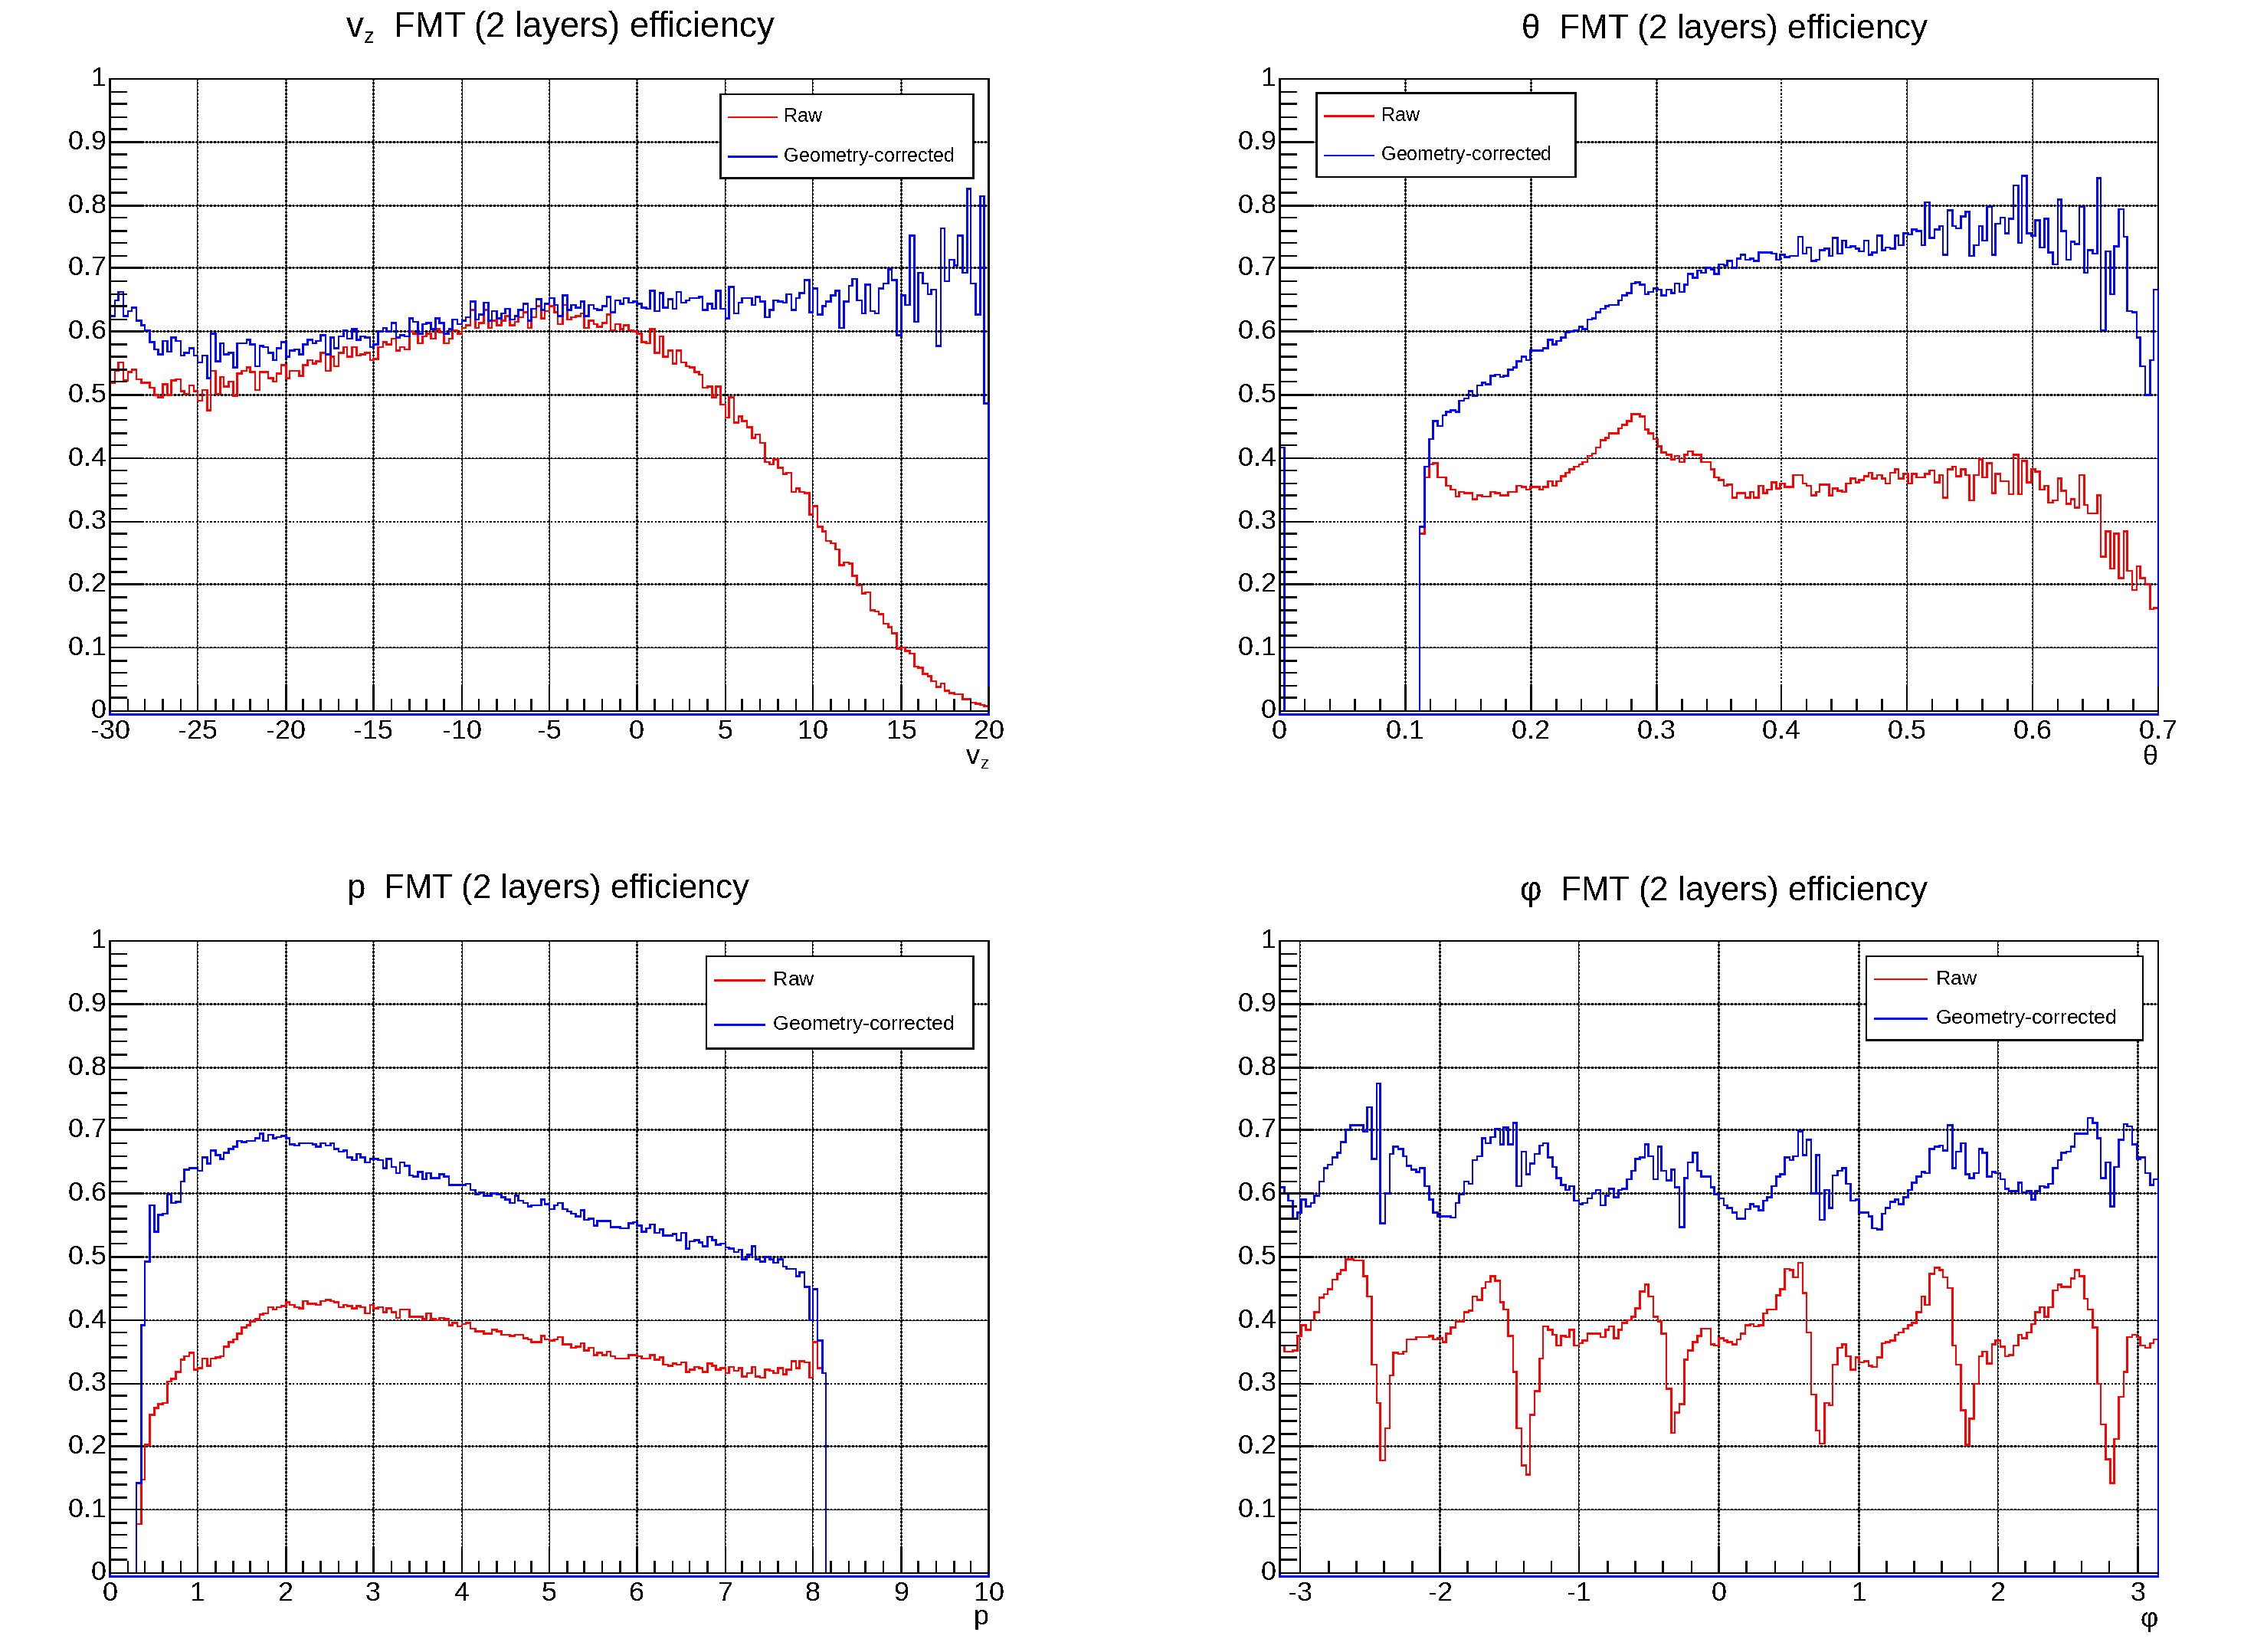
\includegraphics[width=\textwidth]{14resultsandconclusions/img/14efficiencies.pdf}}
        \caption[$v_z$, $\theta$, $\phi$, and $p$ efficiencies for FMT tracks, run 12016]{$v_z$, $\theta$, $\phi$, and $p$ efficiencies for FMT tracks. FMT Efficiency is defined as the percentage of DC tracks that are detected by 2 FMT layers. Run 12016.}
        \label{fig::fmt_efficiencies}
    \end{figure}
